\section{Video management overview}
\label{sec:Video_management_overview}

X-Learning is an e-learning platform that allows users to follow / create courses.
Each course is characterized by a category of interest, description, cost, educational materials and a set of lessons.

%%%%
In general we can split the users into teacher and student, the first of them can be create courses and the secodno of them can benefit from the lessons and teaching materials made available.
%%%%

\subsection{Course management}
\label{sec:course_management}

The creation of the course is articulated in two main phases:

\begin{itemize}
\item The first phase included information such as title, description, language, cost, category, objectives and requirements needed to understand the content. Created course the first phase may be considered completed. Subsequently the teacher will begin the second phase, which consists of adding video lecture and educational content.

\begin{figure}[htb]
 \centering
 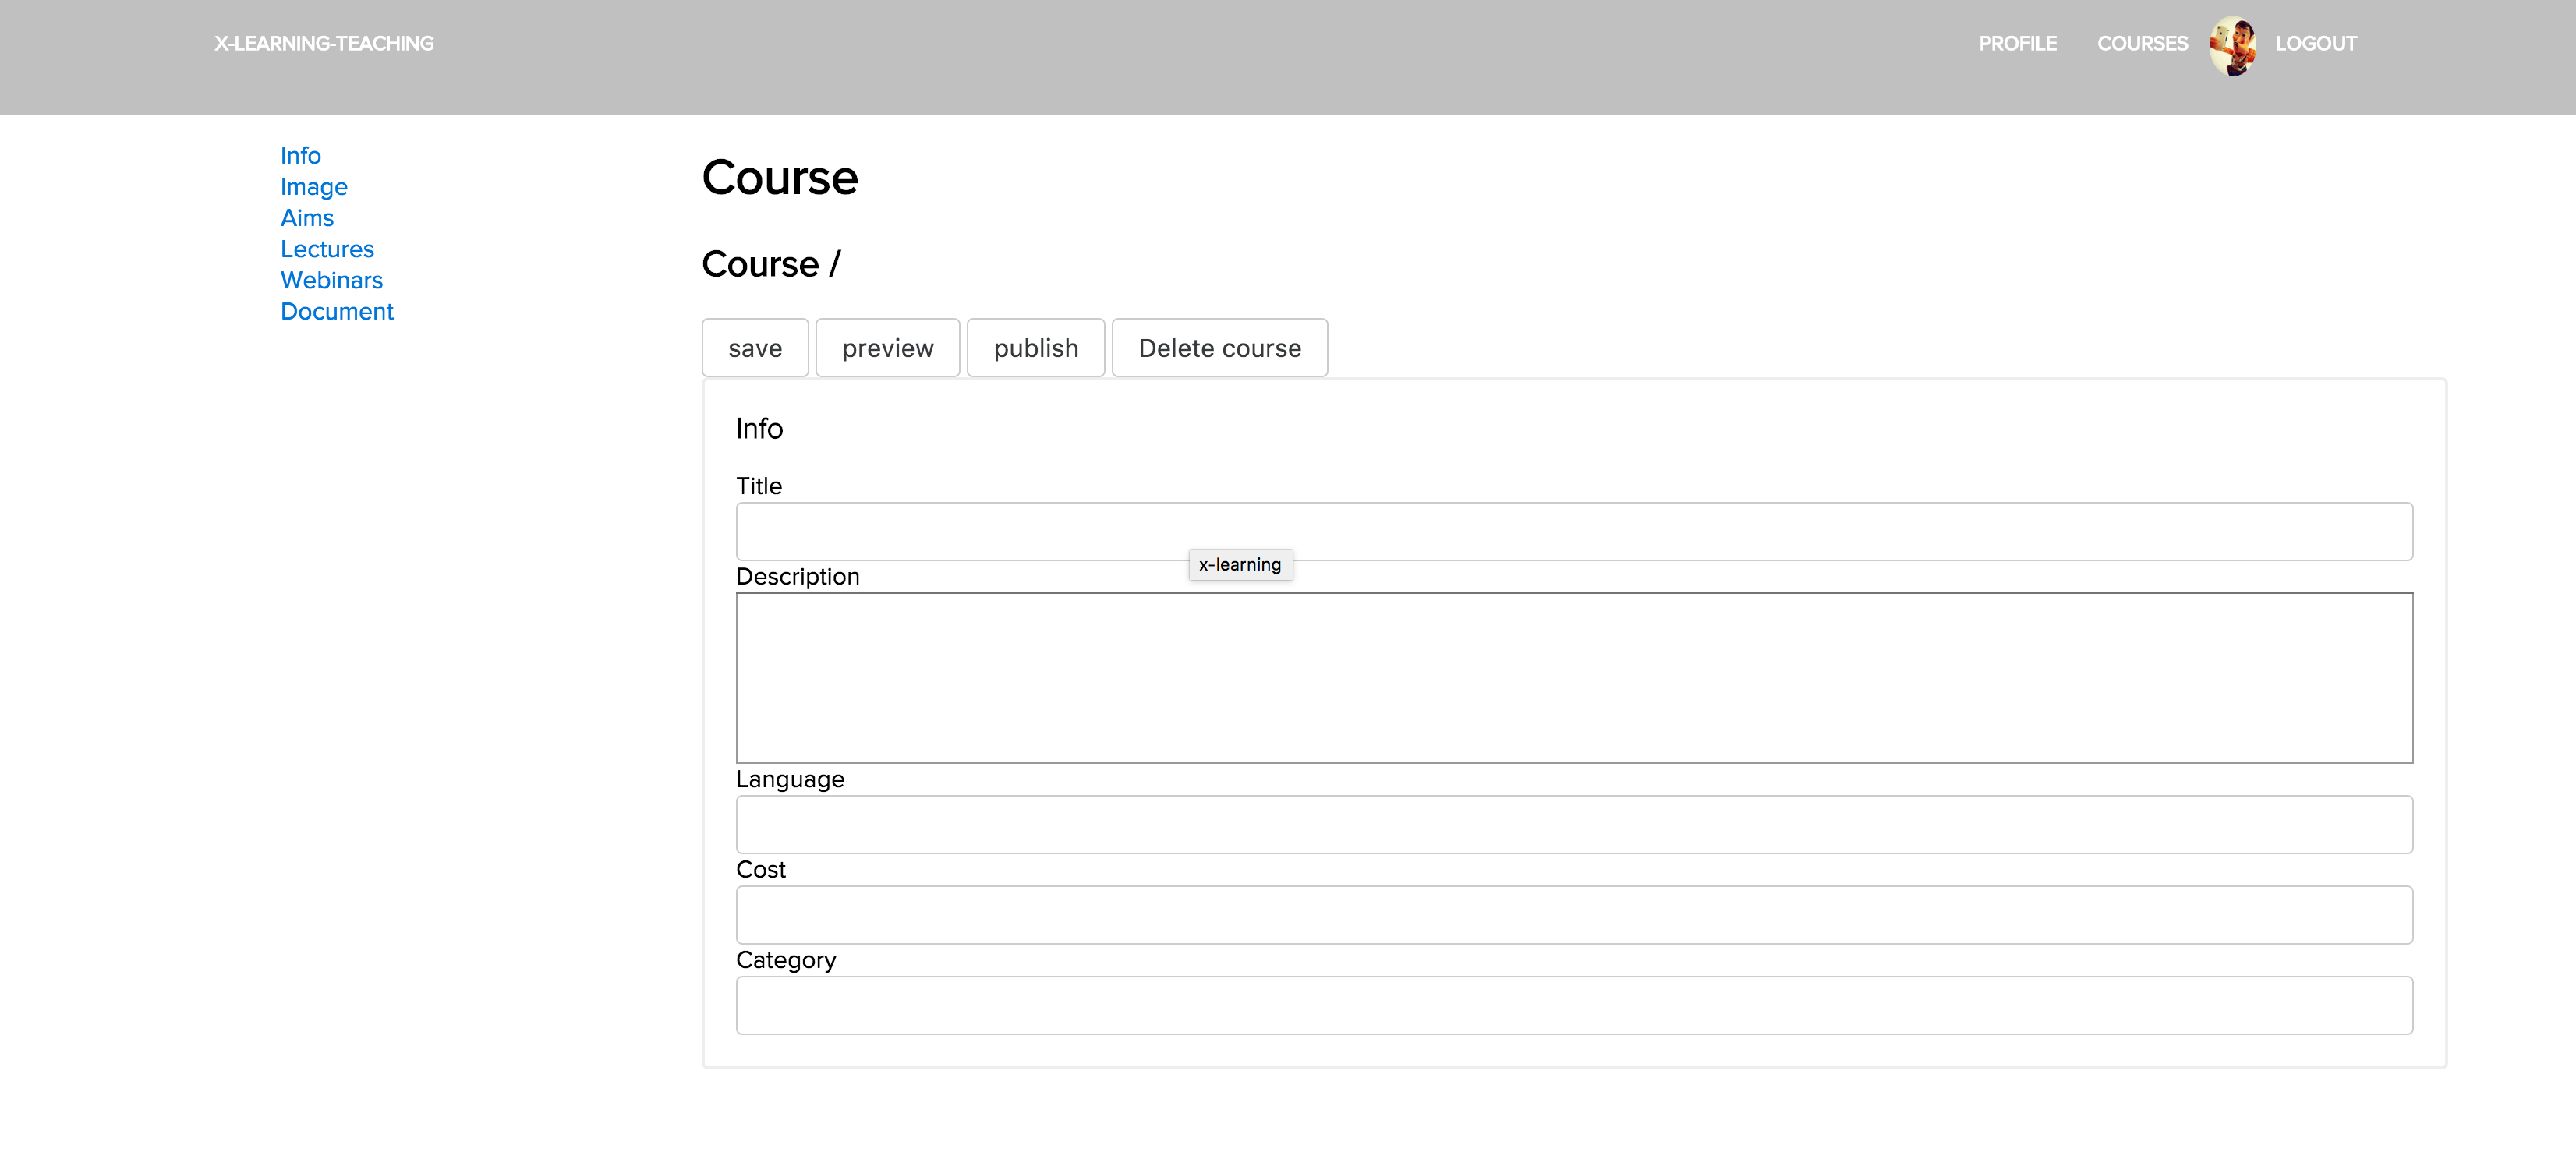
\includegraphics[width=1.0\linewidth]{images/chapter6/insert_course_page.png}\hfill
 \caption[Admin page course]{Admin page course}
 \label{fig:fourV}
\end{figure}

\item The second phase begins with the creation of the lectures, each of which will have a title, a description, and multimedia content.
The page displayed in the picture allows the teacher to select the video that will be associated with the current lesson.

\begin{figure}[htb]
 \centering
 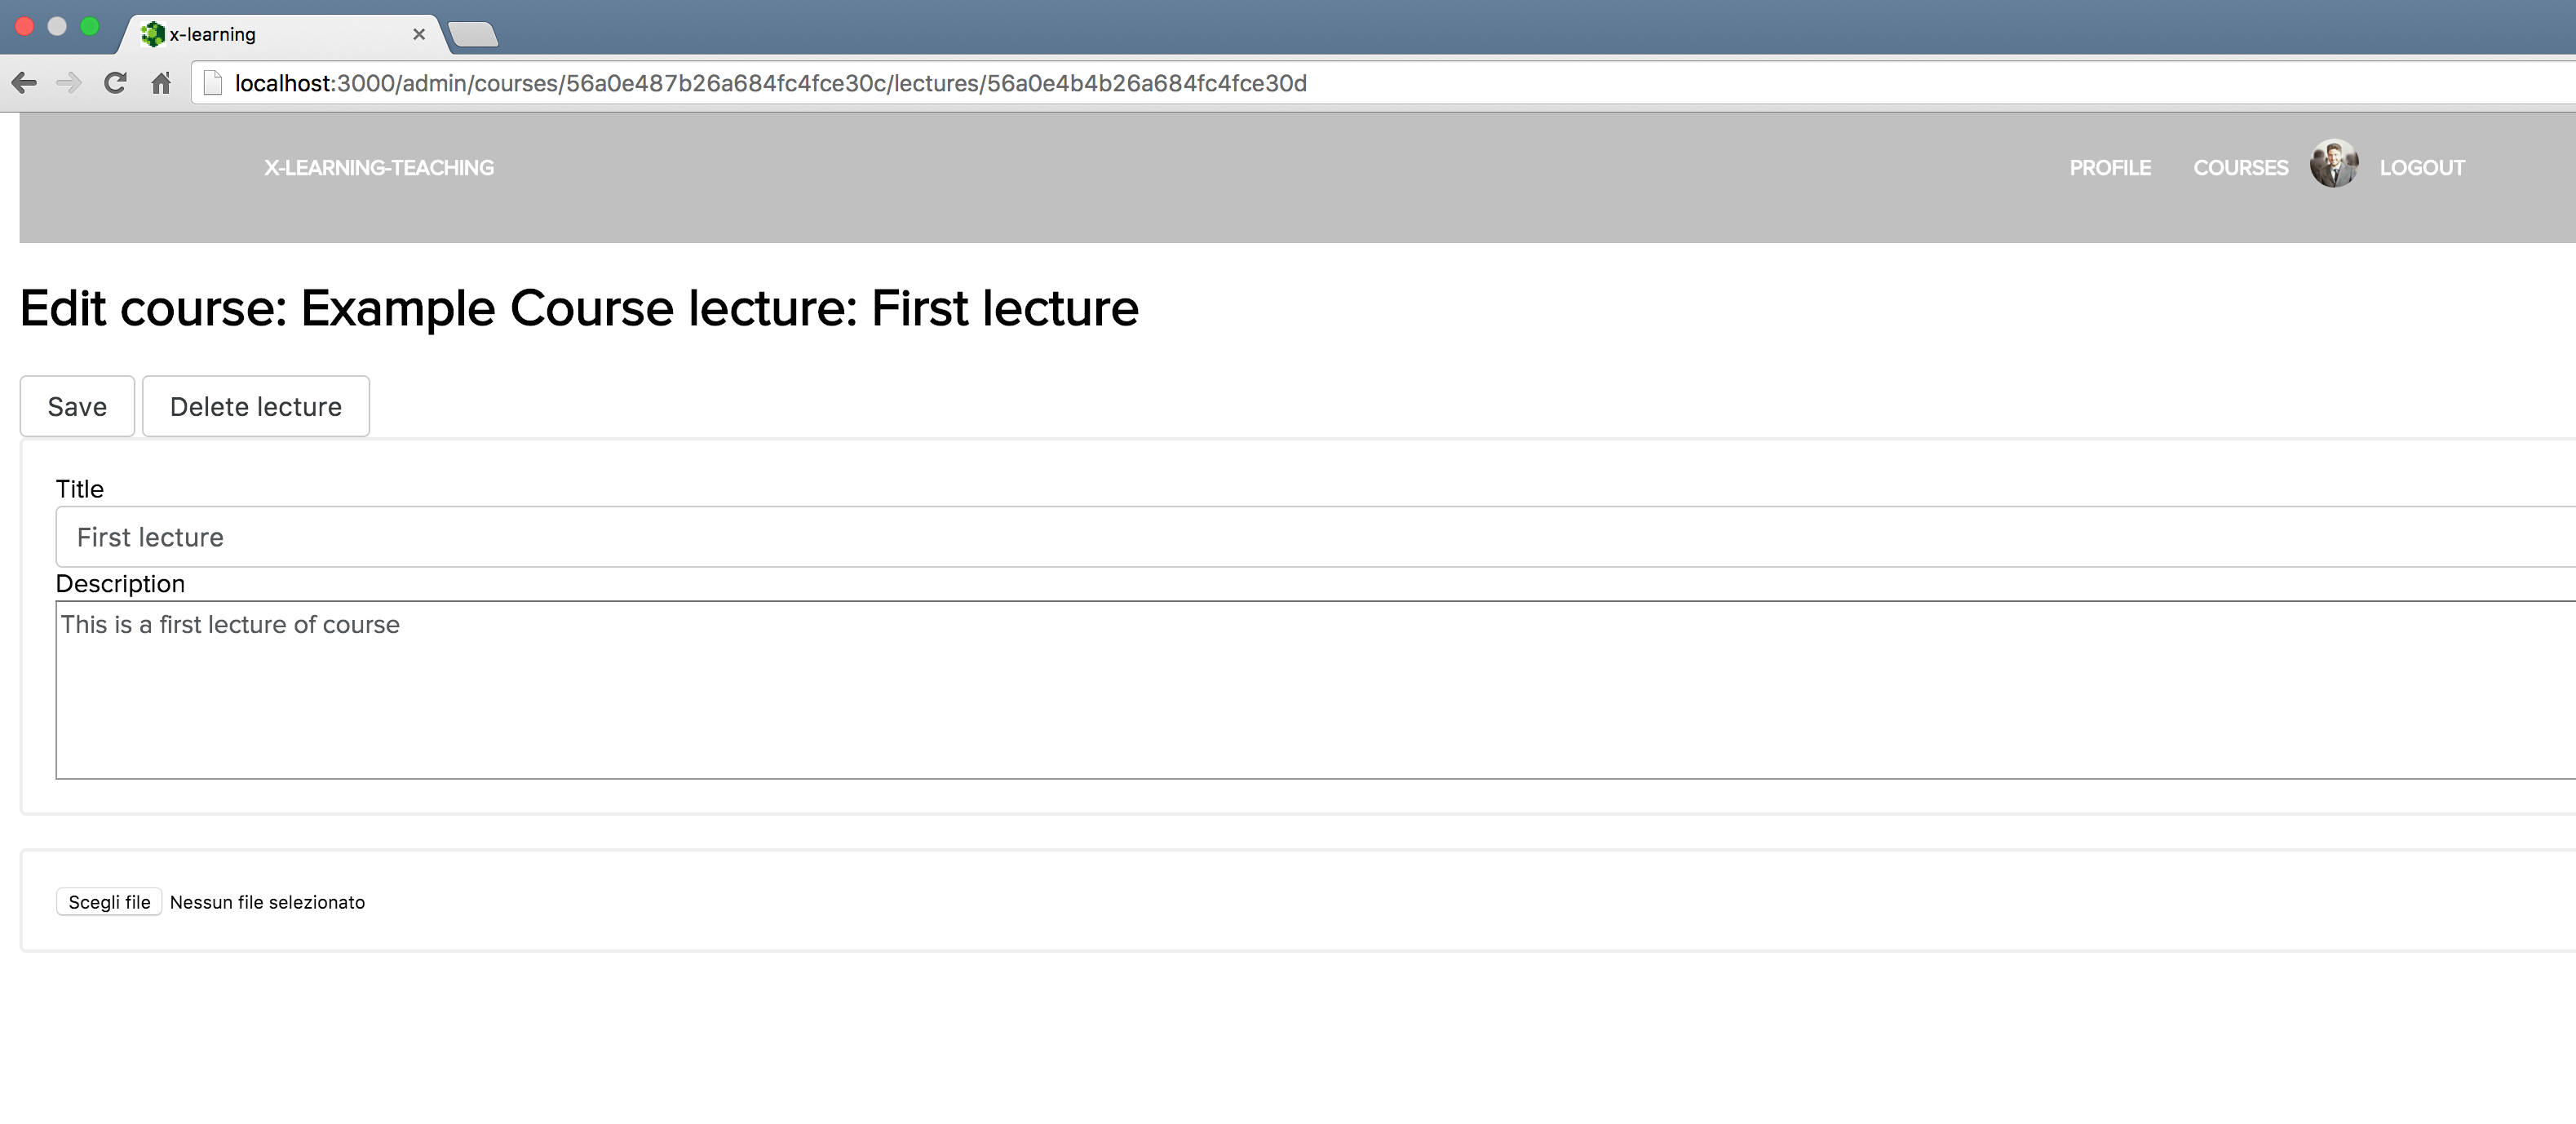
\includegraphics[width=1.0\linewidth]{images/chapter6/insert_lecture.png}\hfill
 \caption[Admin page lecture]{Admin page lecture}
 \label{fig:fourV}
\end{figure}

\end{itemize}

In order to allow upload the video on the client has been created side a web component follows:

\begin{lstlisting}[language=html]
      <input-s3-video></input-s3-video>
\end{lstlisting}

The following tag is responsible for the overall management of uploading and transcoding of video and allows you to enter any work on the project Uploading Videos hiding the full complexity that will be clarified in the following paragraphs.

\subsection{Attend the course}
\label{sec:attend_the_course}
Through the platform of e-learning, the student will find their own course of interest selecting it from those available.
The user chosen and eventually paid the course,then he can start his training.
Also for streaming it has created a web component that allows the video vision, hiding all  encountered problems on the thesis work and complexity that shown in chapter 3.

\begin{lstlisting}[language=html]
       <deck-video src="{{data.lecture.video.url}}"></deck-video>
\end{lstlisting}

The final result will be a player to stream video content as you can see in the picture

\begin{figure}[htb]
 \centering
 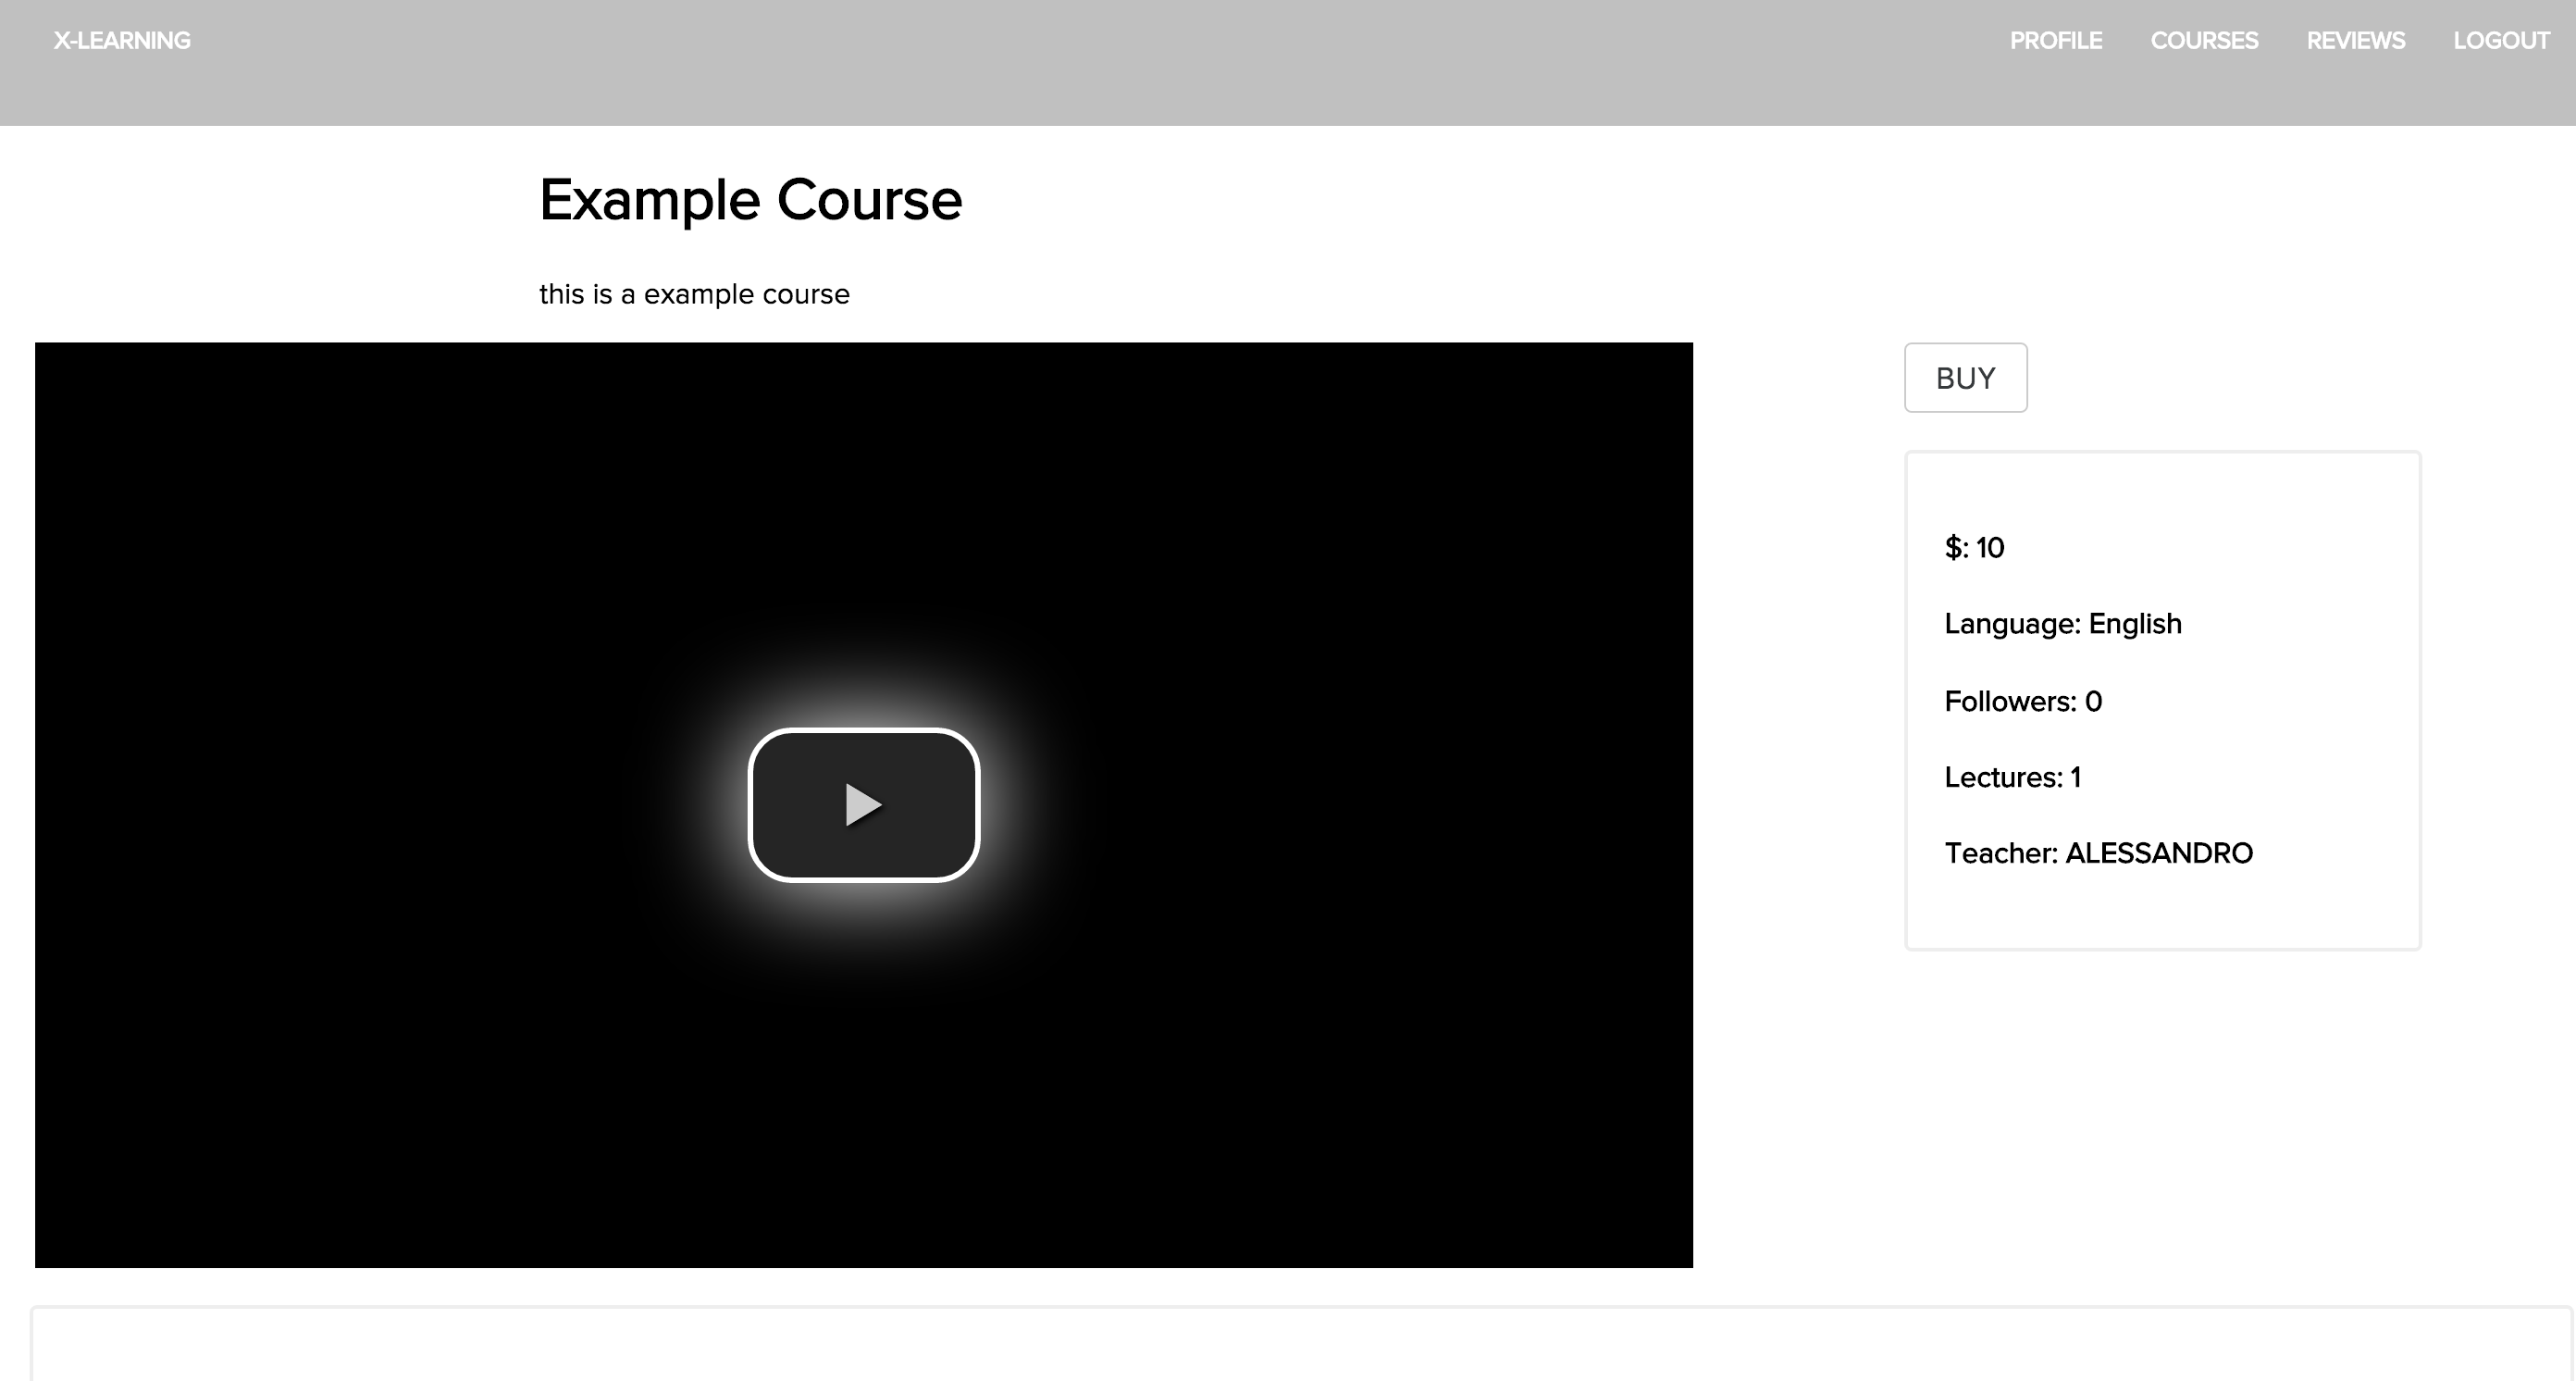
\includegraphics[width=1.0\linewidth]{images/chapter6/deck_video.png}\hfill
 \caption[Deck video]{Deck video}
 \label{fig:fourV}
\end{figure}
